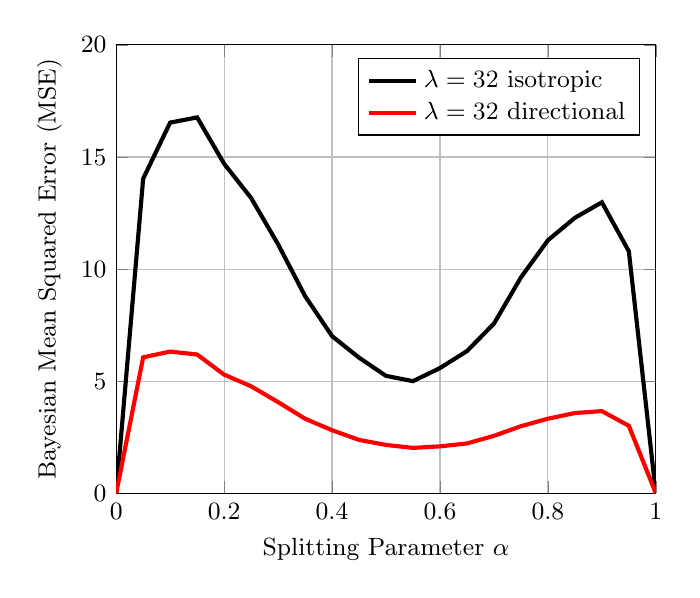
\begin{tikzpicture}
\begin{axis}[
font=\small,
xlabel= {Splitting Parameter $\alpha$},
ylabel= {Bayesian Mean Squared Error (MSE)},
xmin = 0, xmax = 1,
ymin = 0, ymax = 20,
xmajorgrids,
ymajorgrids,
legend entries={$\lambda=32$ isotropic,$\lambda=32$ directional},
legend style={legend pos=north east,nodes=right}]

% Method: Bayes,
% Area Type = inscribed,
% Antenna Type = omnidirectional,
% Noise = 2,
% Trials = 50000,
% Total rate = 16,
% alpha_step =0.025,
% A_t =36.0,
% A_o =64.0,
% BMSE

\addplot [
color=black,
line width=1.5pt,
solid,
]
coordinates{
(0,0.00000000e+00)
(0.05,1.40340910e+01)
(0.1,1.65337525e+01)
(0.15,1.67666833e+01)
(0.2,1.46989584e+01)
(0.25,1.31718747e+01)
(0.3,1.11062848e+01)
(0.35,8.79609488e+00)
(0.4,7.01012537e+00)
(0.45,6.04878165e+00)
(0.5,5.23534228e+00)
(0.55,5.00003850e+00)
(0.6,5.58474031e+00)
(0.65,6.34015503e+00)
(0.7,7.56575455e+00)
(0.75,9.62538999e+00)
(0.8,1.12850060e+01)
(0.85,1.22863272e+01)
(0.9,1.29794969e+01)
(0.95,1.07916156e+01)
(1,1.63496156e-30)
};

% Method: Bayes,
% Area Type = inscribed,
% Antenna Type = directional,
% Noise = 2,
% Trials = 50000,
% Total rate = 16,
% alpha_step =0.025,
% A_t =36.0,
% A_o =64.0,
% BMSE


\addplot [
color=red,
line width=1.5pt,
solid,
]
coordinates{
	(0,0.00000000e+00)
	(0.05,6.06211129e+00)
	(0.1,6.31985246e+00)
	(0.15,6.18877686e+00)
	(0.2,5.29187935e+00 )
	(0.25,4.77082541e+00)
	(0.3,4.06549571e+00)
	(0.35,3.32541741e+00)
	(0.4,2.81081943e+00)
	(0.45,2.37943353e+00)
	(0.5,2.15498374e+00)
	(0.55,2.02272270e+00)
	(0.6,2.09148122e+00)
	(0.65,2.22126422e+00)
	(0.7,2.56077071e+00)
	(0.75,2.98972505e+00)
	(0.8,3.32440510e+00)
	(0.85,3.57826746e+00)
	(0.9,3.66298963e+00)
	(0.95,3.00728985e+00)
	(1,1.66676843e-30)
};

\end{axis}

\end{tikzpicture}

